\documentclass[a4paper, 12pt]{ctexart}

\usepackage[inkscapelatex=false]{svg}

\usepackage{enumitem} 
\usepackage{lmodern}
\usepackage{zhnumber}
\usepackage{graphicx}
\usepackage{geometry}
\geometry{a4paper, top=2.54cm, bottom=2.54cm, left=1.91cm, right=1.91cm}
\usepackage{tocloft} %模板中用了subfigure,不加此选项会产生冲突
\renewcommand{\cftsecleader}{\cftdotfill{\cftdotsep}}
\renewcommand{\contentsname}{\hfill\bfseries 目\quad 录\hfill}

\usepackage{hyperref}
\hypersetup{colorlinks = true, linkcolor = red}

\usepackage{tcolorbox}% 默认加载 pgf、verbatim、environ 宏包
\tcbuselibrary{skins}% 加载 tikz 宏包,并为彩色盒子的外观提供附加样式(外观);
\tcbuselibrary{breakable}% 支持盒子从一个页面自动拆分到另一个页面
\tcbuselibrary{minted}% 排版代码 xelatex -shell-escape main.tex

% set c++
\usepackage{relsize}
\usepackage{xspace}
\protected\def\Cpp{{C\nolinebreak[4]\hspace{-.05em}\raisebox{.28ex}{\relsize{-1}++}}\xspace} 

\definecolor{terminalColor}{RGB}{38,50,56}
\definecolor{Button1}{RGB}{254,94,86}
\definecolor{Button2}{RGB}{254,188,45}
\definecolor{Button3}{RGB}{38,202,59}

\renewcommand{\theFancyVerbLine}{
    % {FancyVerbLine} 表示当前行号的计数器
    \textcolor{white}{\large \arabic{FancyVerbLine}}
}

% pygmentize -L lexers
% c、cpp、bash
% rust、go(golang)、glsl
% cmake、csharp、cuda
% java、javascript、json
% lua、tex、latex
% tex
\def\makecode#1#2#3{
    \newtcblisting{#1} {
        listing engine=minted,
        minted options={linenos=true, numbersep=-6pt},
        minted style=native,
        minted language=#2,
        enhanced,
        colback=terminalColor,
        colframe=terminalColor,
        listing only,
        center,
        width=0.90\textwidth,
        title={
            {
                \raggedright
                {
                    {
                        \tikz {
                            \node[circle,fill=Button1,inner sep=3pt] (c) at (0,0){};
                            \node[circle,fill=Button2,inner sep=3pt] (c) at (0.5,0){};
                            \node[circle,fill=Button3,inner sep=3pt] (c) at (1,0){};
                        }
                    }
                    \hfill
                    {
                        \centering
                        #3
                    }
                    \hfill
                }
            }
        }
    }
}

\makecode{pythoncode}{python}{Python}
\makecode{ccode}{c}{C}
\makecode{cppcode}{cpp}{\Cpp}
\makecode{GCCcode}{cpp}{GCC}

\title{绘制一个三角形}
\author{Zitai-谢雨君}
\date{\today}

\begin{document}

\maketitle

\clearpage
\tableofcontents

\clearpage
\section{写在前面}
    相比于 OpenGL,Vulkan 为我们提供了更广阔的自由空间;
    与此同时,也需要开发者自己管理更多更细节的东西。
    本文以绘制一个三角形为例,简单剖析一个大致完整的 Vulkan 程序运行流程。

    程序核心内容分为四各部分:

    \begin{enumerate}[itemindent=1em, itemsep=0pt, topsep=0pt, parsep=0pt]
        \item \textbf{初始化屏幕窗口};
        \item \textbf{初始化 Vulkan 相关设置};
        \item \textbf{进入事件主循环};
        \item \textbf{清理资源并退出}。
    \end{enumerate}




\clearpage
\section{初始化屏幕窗口}
    Vulkan 是一个底层的图形 API,若想实时输出图像到窗口,
    需要开发者自己编写大量与平台操作系统相关的代码来处理窗口创建、用户输入、上下文管理等底层操作。
    而 GLFW、SDL 等库可以提供封装好的接口来处理这些底层操作,简化了 Vulkan 开发的流程,
    使得开发者能够更加专注于图形渲染的实现。
    这里使用 GLFW 来管理窗口。
    
    \href{https://www.glfw.org/}{GLFW} 是一个开源、多平台的库,
    用于 OpenGL、OpenGL ES 和 Vulkan 在桌面上的开发。
    它提供了简单的 API,用于创建窗口、上下文和表面,接收输入和事件。
    GLFW 是用 C 编写的,支持 Windows、macOS、X11 和 Wayland。

    在创建窗口前,必须先使用 \texttt{glfwInit} 函数来初始化 GLFW 库,
    并且在应用程序终止之前,释放分配的资源。
    如果初始化失败,该函数会在返回前调用 glfwTerminate 函数;
    如果成功,就需要在应用程序返回前手动调用 glfwTerminate 函数。

    接着使用 \texttt{glfwWindowHint} 函数为 \texttt{glfwCreateWindow} 的调用设置提示。
    提示一旦设置,将保留其值,直到通过调用此函数或 \texttt{glfwDefaultWindowHints} 进行更改,或者直到库终止。
    hints 分为硬约束和软约束。
    因为 Vulkan 和 OpenGL 上下文是相互独立的,
    所以需要明确指示 GLFW 不要为窗口创建 OpenGL 上下文,从而为 Vulkan 渲染留出空间。
    因此需要调用 \texttt{glfwWindowHint(GLFW\_CLIENT\_API, GLFW\_NO\_API)} 函数。
    
    接下来就可以调用 \texttt{glfwCreateWinow} 函数来创建一个窗口。

    这部分代码较为简单:

\begin{cppcode}
 glfwWindowHint(GLFW_CLIENT_API, GLFW_NO_API);
 glfwWindowHint(GLFW_RESIZABLE, GLFW_FALSE);// 禁止改变窗口大小
 GLFWwindow* window =
     glfwCreateWindow(800, 600, "Hello Window", nullptr, nullptr);
\end{cppcode}
    
    其中,GLFWwindow 对像是窗口和上下文的封装。
    窗口和上下文是不可分割的链接,对象指针同时用作上下文和窗口句柄。




\clearpage
\section{初始化 Vulkan 相关设置}
\subsection{实例}
    在 Vulkan 中不再需要依赖于绑定在某个线程上的 Context 全局状态,
    所有应用程序的状态都存储在相应的 VkInstance 对象(一般称为实例)中。
    VkInstance 是一切 Vulkan 函数的源头,一个进程(应用程序)只拥有一个 VkInstance。
    编写应用程序的第一步是创建实例来初始化 Vulkan library。
    实例是应用程序与 Vulkan 库之间连接的桥梁,VkInstance 对象存储每个应用的状态。
    
    在创建过程中,通常需要向驱动程序提供一些应用程序自身的信息。
    当然,这些信息的填写不是必须的,但填写的信息可以作为驱动程序的优化依据,让驱动程序进行一些特殊的优化。

    基本的 Vulkan 架构看起来像这样:

    \begin{figure}[htbp]
        \centering
        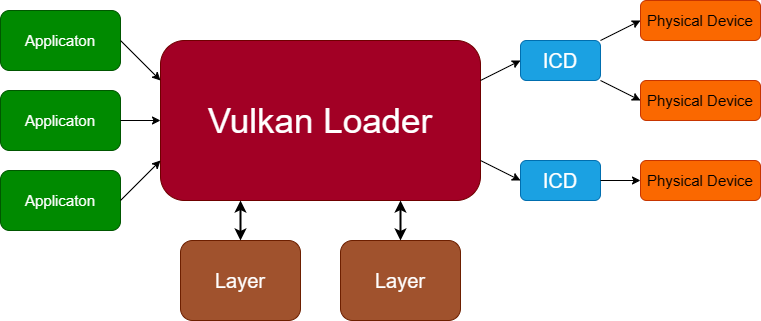
\includegraphics[scale = 0.6]{images/Instance.png}
        \caption{Vulkan 应用程序架构}
    \end{figure}

    图中的 Layer 也通过 Loader 加载,Layer 通常用于验证,是由驱动执行的错误检查。
    Vulkan 的驱动程序比 OpenGL 等其他 API 要轻量得多,部分原因是它将功能验证委托给 Validation Layer。
    Layer 是可选的,应用程序创建 VkInstance 时可以根据需求选择性地装载 Layer。

    Layer 总的来说是增强 Vulkan 系统的可选组件。
    它们可以在从应用程序到硬件的过程中拦截、评估和修改现有的 Vulkan 功能。
    可以使用 \texttt{vkEnumerateInstanceLayerProperties} 函数从应用程序中查询可用的 Layer 的属性。
    
    \texttt{VkApplicationInfo} 结构体为实例赋予自定义应用程序的信息,这些数据是可选的。

    \texttt{VkInstanceCreateInfo} 结构体是必须而不是可选的,
    使用它告知 Vulkan 驱动程序我们需要使用哪些全局的 extensions 和 validation layers。
    这里的全局意味着它适用于整个程序,而不是特定的设备。


\clearpage
\subsection{校验层}
    Vulkan API 的设计是围绕最小化驱动程序开销进行的,
    所以,默认情况下,Vulkan API 提供的错误检查功能非常有限,因此,Vulkan 引入校验层来解决这个问题。
    校验层是一个可选的、用来在 Vulkan API 函数调用上进行附加操作的组件。
    校验层常被用来做下面的工作:

    \begin{itemize}[itemindent=1em, itemsep=0pt, topsep=0pt, parsep=0pt]
        \item 检测参数值是否合法;
        \item 追踪对象的创建和清除操作,发现资源泄露问题;
        \item 追踪调用的线程,检测是否线程安全;
        \item 将 API 调用和调用的参数写入日志;
        \item 追踪 API 调用进行分析和回放。
    \end{itemize}

    这些 Validation layers 可以随意的堆叠到 Vulkan 驱动程序中\footnote{
        在之前的 Vulkan 版本中有两种不同类型的 Validation layers,
        分别应用于 instance 和 device specific。
        这个设计理念希望 instance 层只会验证与全局 Vulkan 对象(例如Instance)有关的调用,
        而 device specific 层只是验证与特定 GPU 相关的调用。
        device specific 层已经被废弃,这意味着 instance 层的 Validation layers 将应用到所有的 Vulkan 调用。
        出于兼容性的考虑,规范文档仍然建议在 device specific 层开启 Validation layers,这在某些情景下是有必要的。
    },
    如果有必要,甚至可以包含所有的 debug 功能。
    可以选择只在应用程序的 debug 版本中开启 Validation layers,
    在 release 版本中禁止,从而提供两个应用程序版本。

    值得一提的是,Vulkan 没有内置任何 Validation layers,
    可以根据你需要的检测需求应用具体的 Validation layers,
    Vulkan 只能使用已经安装到系统上下文的 Validation layers。
    例如,LunarG Validation layers 仅在安装了 Vulkan SDK 的 PC 上可用。


    % auto func = (PFN\_vkCreateDebugReportCallbackEXT) vkGetInstanceProcAddr(instance, "vkCreateDebugReportCallbackEXT");

    % 所有 Vulkan 命令的函数指针都可以通过 vkGetInstanceProcAddr 来获取。
    % 这行代码的作用是获取 Vulkan 实例中的 vkCreateDebugUtilsMessengerEXT 函数的地址,
    % 并将其存储在名为 func 的函数指针变量中,该函数指针的类型为 PFN\_vkCreateDebugUtilsMessengerEXT。
    
    % PFN\_vkCreateDebugUtilsMessengerEXT 是一个函数指针的类型,
    % 它定义了一个指向 vkCreateDebugUtilsMessengerEXT 函数的指针。
    % 在 Vulkan 应用程序中,通常会使用 vkGetInstanceProcAddr 函数来获取 Vulkan 实例中函数的地址,并将其转换为函数指针。

    % 在 Vulkan 中既可以通过函数指针来调用函数,也可以直接调用函数。
    仅仅启用校验层并没有任何用处,因为我们不能得到任何有用的调试信息。
    为了获得调试信息,还需要使用 VK\_EXT\_debug\_utils 扩展,设置回调函数来接受调试信息。


\clearpage
\subsection{物理设备和队列族}
    Vulkan 分离了物理设备和逻辑设备的概念。
    物理设备通常代表主机中一个可用的 Vulkan 完整实现\footnote{简单理解为一个物理设备对应一张显卡,其数量有限}。
    逻辑设备代表该实现的一个实例,具有独立于其他逻辑设备的状态和资源。
    
    \textbf{总结}:一个 VkInstance 对应一个或多个有限的 VkPhysicalDevice;
    一个 VkPhysicalDevice 对应一个或多个 VkDevice。
    
    通过 VkInstance 初始化 Vulkan library 后,
    需要在系统中查找并选择一个支持我们所需功能的硬件设备(显卡)。
    实际上,也可以选择任意数量的显卡并同时使用他们。

    Vulkan 中的几乎所有与 GPU 相关的操作,都需要将命令提交到 Queue,然后才能执行。
    一个物理设备能支持一个或多个不同的队列族,每个队列族都支持一种或多种队列(例如,图形队列,呈现队列)。
    VkQueue 可以支持各种类型的操作,“队列族”只是一个描述一组具有公共属性并支持相同功能 VkQueue 的集合。
    因此,不同 QueueFamilies 有不同的属性,并且每个 QueueFamilies 的 Queue 只允许执行特定的一部分指令。
    例如,可能存在只允许执行计算相关指令的队列族和只允许执行内存传输相关指令的队列族。
    我们需要检查设备支持哪些类型 QueueFamilies,以及其中哪一个支持我们想要使用的命令,
    从而挑选出适合我们应用程序的物理设备。

    每个队列族都有一个唯一的队列族索引(Queue Family Index)来标识它。
    每个队列族中可以有一个或多个队列,每个队列都有一个唯一的队列索引(Queue Index)来标识它。
    队列按照提交的命令顺序执行渲染和计算操作。
    使用多个队列,可以增加并发,使用特定队列可以提升性能。

    \texttt{VkQueueFamilyProperties} 结构体描述了队列的特性,其中值得注意的是 queueFlags 成员变量。
    在 Vulkan 中,很多“描述性”的结构体中都有一个 flags 变量,它是另一个相关枚举类型的掩码(bitmask),
    例如这里的 queueFlags 就是 VkQueueFlagBits 枚举类型的掩码。
    VkQueueFlagBits 枚举类型包含了很多枚举值,例如,
    
    \begin{itemize}[itemindent=1em, itemsep=0pt, topsep=0pt, parsep=0pt]
        \item VK\_QUEUE\_GRAPHICS\_BIT = 0x00000001
        \item VK\_QUEUE\_COMPUTE\_BIT = 0x00000002
        \item VK\_QUEUE\_TRANSFER\_BIT = 0x00000004
        \item VK\_QUEUE\_SPARSE\_BINDING\_BIT = 0x00000008
    \end{itemize}

    想要检查 VkPhysicalDevice 的队列族是否支持图形队列时,
    可以用 queueFlags 掩码与 VK\_QUEUE\_GRAPHICS\_BIT 作 \& 运算
    \footnote{
        掩码是十进制,枚举值是十六进制,将它们都转换为二进制再作 \& 运算。
    },
    如果结果是 1 则表示支持,反之不支持。
    估计这样的设计是用来简化代码。

    在 Vulkan 中,可以创建一个图形队列族和一个计算队列族。
    这样的创建方式与将这两个队列创建在同一个队列族中有以下区别:

    \begin{itemize}[itemindent=1em, itemsep=0pt, topsep=0pt, parsep=0pt]
        \item 独立的队列族:创建独立的图形队列族和计算队列族意味着它们是完全独立的,彼此之间没有任何关联。
                它们具有不同的队列标识和特性,并且可以单独进行操作和调度。
        \item 资源隔离:将图形队列和计算队列分别创建在不同的队列族中,可以更好地隔离它们所使用的资源。
                由于图形操作和计算操作通常具有不同的资源需求,如缓冲区、纹理等,
                将它们分开可以更好地管理和优化这些资源的分配和使用。
        \item 灵活性和控制:将图形队列和计算队列分开创建可以提供更大的灵活性和控制。
                例如,如果应用程序需要更多的图形处理能力,可以通过增加图形队列的数量来满足需求,而不会对计算队列产生影响。
                同样,如果需要更多的计算能力,可以独立地增加计算队列的数量。
        \item 任务调度:将图形队列和计算队列分开创建还可以更好地进行任务调度。
                由于图形操作和计算操作具有不同的特性和优化需求,
                将它们分开可以更好地进行任务的调度和执行,以最大限度地提高性能。
    \end{itemize}


\clearpage
\subsection{逻辑设备}
    逻辑设备(logical device)对象表示到物理设备的逻辑连接。
    % 每个物理设备都公开了许多队列族,每个队列族都有一个或多个队列。
    % 一个队列族中的所有队列都支持相同的操作。

    Vulkan 应用程序将首先查询系统中的所有物理设备,
    然后查询每个物理设备的能力,包括它的队列和队列族属性。
    一旦识别出可接受的物理设备,应用程序就会创建相应的逻辑设备。
    然后,创建的逻辑设备就是物理设备的主接口。

    % 如果多个物理设备属于同一个设备组,则可以从这些物理设备创建单个逻辑设备。
    % 设备组是一组物理设备,支持访问彼此的内存并记录可以在所有物理设备上执行的单个命令缓冲区。
    % 通过调用 \texttt{vkEnumeratePhysicalDeviceGroups} 来枚举设备组,
    % 并且通过将物理设备传递给 \texttt{VkDeviceGroupDeviceCreateInfo} 来从设备组中的物理设备的子集创建逻辑设备。
    % 要使两个物理设备位于同一设备组中,它们必须支持相同的扩展、功能和属性。

    逻辑设备创建过程与 VkInstance 创建过程类似,也需要描述我们需要使用的功能。
    因为已经查询过哪些 QueueFamily 可用,
    在这里需要进一步为逻辑设备创建具体类型的 Command Queue。
    如果有不同的需求,也可以基于同一个物理设备创建多个逻辑设备。

    我的理解是,一个物理设备提供了多个队列,
    我们可以根据这些队列组合成不同的队列族,将不同的队列族绑定不同的逻辑设备时,
    就组合成了不同的逻辑设备。


\clearpage
\subsection{交换链}
    每一个支持显示的平台都有自己的窗口系统(Windowing System Integration, WSI)。
    Vulkan 提供了 Swap Chains 跟平台的窗口系统对接。
    
    在 Vulkan 中,使用交换链(swap chain)作为将渲染图像提交到屏幕的基本机制,
    它需要在 Vulkan 上下文中被明确创建。
    从屏幕的角度观察,交换链本质上是一个图像队列。
    应用程序作为生产者会获取图像进行绘制,然后将其返还给交换链图像队列,等待屏幕消费。
    交换链的具体配置信息决定了应用程序提交绘制图像到队列的条件以及图像队列呈现的效果,
    但通常使用交换链的目的是使绘制图像的最终呈现与屏幕的刷新频率同步。
    可以简单将交换链理解为一个队列,同步从生产者,即应用程序绘制图像,到消费者,屏幕刷新的 Produce-Consume 关系。

    \begin{figure}[htbp]
        \centering
        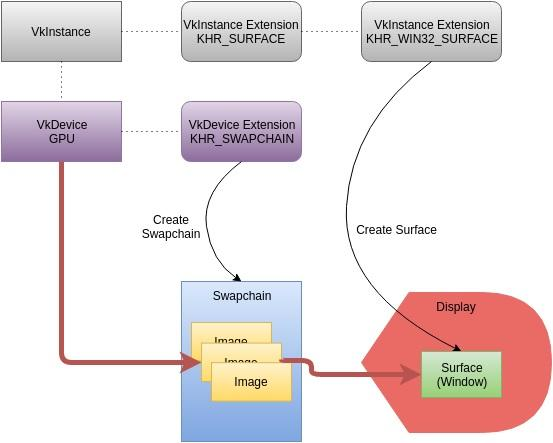
\includegraphics[scale = 0.6]{images/swapchain.jpg}
        \caption{swap chain}
    \end{figure}
    
    Swap Chain 会向窗口系统申请一个或者多个可以用于显示的 VkImage 对象。
    我们可以将这些 image 对象作为我们的绘制目标,绘制完成后通过 \texttt{vkQueuePresentKHR} 函数送显。


\clearpage
\subsection{窗口表面}
    当使用 OpenGL 时,可以使用 GLFW 来创建窗口和处理用户输入等操作。
    GLFW 封装了底层的窗口系统,并提供了一些方便的函数来创建和管理窗口。
    因为 OpenGL 是较为高级的 API,它隐藏了许多与窗口系统交互的细节,所以 GLFW 可以直接创建和管理窗口。

    而当使用 Vulkan 时,由于其底层和高性能的特性,它需要更多的控制和配置。
    Vulkan 需要与窗口系统进行更直接的交互,并且需要将图形渲染的结果显示在窗口上。
    为了实现这个过程,Vulkan 引入了窗口表面(Surface)的概念。
    所以在使用 Vulkan 时,即使采用了 GLFW,仍然需要处理窗口表面的创建和管理。

    窗口表面是一个用于显示图形渲染结果的抽象概念,它代表了与窗口系统交互的接口。
    在 Vulkan 中,需要通过窗口表面来创建交换链(Swapchain),交换链用于管理渲染图像的呈现和刷新。
    窗口表面的创建需要与特定的窗口系统进行交互,因此需要使用 GLFW 等库来完成这个过程。

    \textbf{总结}:交换链(Swapchain)是用于在窗口系统和图形设备之间进行图像交换的机制。
    它是一组用于显示图像的帧缓冲区,用于在绘制完成后将图像呈现到屏幕上。
    表面窗口是与窗口系统相关的对象,它表示一个可绘制的表面,用于将图像渲染到屏幕上。


\clearpage
\subsection{图像}
    VkImage 是 Vulkan 中用于表示图像数据的对象。
    它是一个抽象的概念,代表了图像在内存中的存储和布局。
    VkImage 对象本身并不存储实际的图像数据,而是描述了图像的各种属性和用途。

    VkImage包含了以下信息:

    \begin{itemize}[itemindent=1em, itemsep=0pt, topsep=0pt, parsep=0pt]
        \item 图像的格式:描述了图像数据的像素格式,如颜色通道的数量、位深度和数据类型等。
        \item 图像的尺寸:描述了图像的宽度、高度和深度(对于3D图像)。
        \item 图像的层数:对于3D图像和立方体贴图等具有多个层级的图像,描述了图像的层数。
        \item 图像的采样级别:对于多级别纹理(mipmap)和抗锯齿图像等具有多个采样级别的图像,描述了图像的采样级别。
        \item 图像的用途:描述了图像在渲染过程中的用途,如作为颜色附件、深度附件、纹理等。
        \item 图像的布局:描述了图像数据在内存中的存储布局,如行主序或块主序等。
    \end{itemize}

    VkImage 对象可以通过调用 Vulkan API 来创建,被用于创建交换链、帧缓冲、纹理等其他 Vulkan 对象。
    在图像的使用过程中,可以通过 VkImageView 对象来引用 VkImage,并对图像进行采样、访问和操作。

    在 Vulkan 中,图像的实际数据存储在 VkDeviceMemory 对象中。
    VkDeviceMemory 是用于表示设备内存的 Vulkan 对象,它用于存储图像数据、缓冲数据和其他资源的实际内容。
    在创建 VkImage 对象时,需要为其分配对应的 VkDeviceMemory 来存储图像数据。
    这可以通过调用 vkAllocateMemory 函数来完成。
    为 VkImage 分配内存后,还需要调用 vkBindImageMemory 函数将其与 VkImage 对象绑定起来。
    一旦 VkImage 对象与 VkDeviceMemory 关联起来,图像数据就会被存储在该内存中。
    之后还需要使用 Vulkan 的内存映射机制,将 VkDeviceMemory 对象映射到主机内存中,以便对图像数据进行读取和写入操作。
    需要注意的是,图像数据的存储布局和格式在 VkImage 对象的创建过程中会被指定,以便在内存中正确地存储和解释图像数据。
    这些信息包括像素格式、尺寸、层数、采样级别等等。

    相关操作流程:创建图像、计算所需内存、分配图像内存、绑定图像和图像内存。


\clearpage
\subsection{图像视图}
    VkImage 不能与渲染管线进行交互,为了在渲染管线中使用任何 VkImage 对象,
    包括 Swap Chain 中的那些 VkImage 对象,必须创建一个 VkImageView 对象。
    VkImageView 实际上是对图像的一种解释,描述了对图像数据的访问和使用方式,定义了图像数据的格式、范围和用途。
    不同的图像视图类型对应于不同的图像维度和数据布局,以满足不同的需求。
    它描述了如何访问图像以及访问图像的哪一部分,只有通过 VkImageView 对象,具体的管线才能够读写渲染数据。
    除此之外,图像视图可以进一步定义具体 VkImage 的格式,
    比如定义为 2D 贴图,那么本质上就不需要任何级别的 mipmapping。

    图像视图不同于图像本身,它是对图像的一种视图或解释方式。
    通过创建不同类型的图像视图,可以以不同的方式访问和操作相同的图像数据,以满足不同的需求和用途。

    图像视图的作用如下:

\begin{itemize}[itemindent=1em, itemsep=0pt, topsep=0pt, parsep=0pt]
    \item 格式转换:图像视图允许你使用不同的格式来访问图像数据。
            例如,你可以将一个RGBA图像以不同的方式解释为红色通道、绿色通道、蓝色通道或透明度通道。
    \item 子区域访问:图像视图可以定义访问图像数据的子区域。这使得你可以只处理图像的一部分,而不需要处理整个图像。
    \item 多样本采样:对于多样本图像(例如,用于抗锯齿),图像视图可以定义如何对多个样本进行采样,以便进行图像处理或渲染。
    \item 纹理采样:图像视图可以用于将图像数据绑定到纹理采样器上,以便在着色器中进行纹理采样和纹理操作。
    \item 渲染目标:图像视图可以用于将图像数据绑定到帧缓冲中的附件(attachment),以供渲染过程中进行渲染操作。
    \item 通过使用图像视图,你可以更灵活地访问和使用图像数据,以满足你的需求。
            它提供了一种在图像层面上进行精细控制的方式,使得图像处理和渲染更加灵活和高效。
\end{itemize}


\clearpage
\subsection{RenderPass}
    RenderPass 是现代图形 API 提出的新概念,
    简单来说 RenderPass 定义了一次渲染操作的整体描述,
    包括颜色、深度和模板附件的加载和存储操作、子传递和依赖关系等。
    一个 RenderPass 通常包含多个子渲染过程(subpass),每个子渲染过程可以包含一系列的绘制命令。
    子渲染过程可以在不同的附件上执行,并且可以有依赖关系,以确保正确的渲染顺序。
    RenderPass 本质是定义一个完整的渲染流程以及对所使用的资源的描述,
    可以理解为是一份元数据或者占位符的概念,其中不包含任何真正的数据。

    在 Vulkan 中,不能在没有 RenderPass 的情况下渲染任何东西。
    而且每个 RenderPass 必须有一个或多个子步骤。
    这些子步骤被称为 SubPass,每个 SubPass 都是使用 RenderPass 中定义的资源描述。
    RenderPass 的资源可能包括 Color、Depth/Stencil、Resolve Attachment 和 Input Attachment\footnote{
        在同一个 RenderPass 中,前一个 SubPass 的输出对于后一个执行的 SubPass 同样属于 RenderPass 的资源
    },而这些资源被称为 Attachment。
    为什么不直接把它们叫做 RenderTarget 呢?
    因为 Attachment 只是资源描述(元数据)定义一些加载/存储操作以及相应资源的格式。
    RenderPass 其实是通过 Framebuffer 中包含的 ImageView 拿到真正的数据(牢记 RenderPass 只是元数据)。
    并且之后的 RenderPass 中只要满足 Vulkan 定义的 Render Pass Compatibility 要求的 Framebuffer,
    Framebuffer 就能通过 RenderPass 渲染出相应的结果。

    其中的 dependencyCount 成员表示与该渲染通道(RenderPass)关联的依赖关系数量。
    依赖关系是指在渲染通道中,一个 SubPass 必须在另一个 SubPass 之前或之后执行的关系。
    依赖关系通常用于描述渲染操作之间的同步和顺序关系,以确保正确的渲染顺序和数据一致性。
    通过设置 dependencyCount 的值,可以告诉 Vulkan 运行时有多少个依赖关系需要考虑和处理。
    在使用 VkRenderPass 时,通常需要创建一个 VkSubpassDependency 结构体的数组,并将其与 VkRenderPass 一起使用。
    每个 VkSubpassDependency 结构体描述了一个依赖关系,包括依赖关系的源子通道、目标子通道、依赖关系的阶段和访问标志等。
    通过设置 dependencyCount 的值,并正确配置 VkSubpassDependency 结构体数组,
    可以定义和管理渲染通道中的依赖关系,以确保正确的渲染顺序和数据同步。

    \textbf{总结}:SubPass 和 RenderPass 都是走一个 pipeline(VS -> TS -> GS -> 光栅化 -> FS),
    只不过多个 SubPass 可以通过 Input Attchment 利用前一个 SubPass 的 output 结果,
    从而直接访问 Tiled Bufferd 的同一处,不需要访问内存;
    而多个 RenderPass 如果要利用前一个 RenderPass 的结果,则需要利用纹理采样的方式访问内存。

    
\clearpage
\subsection{渲染管线}
    \begin{figure}[htbp]
        \centering
        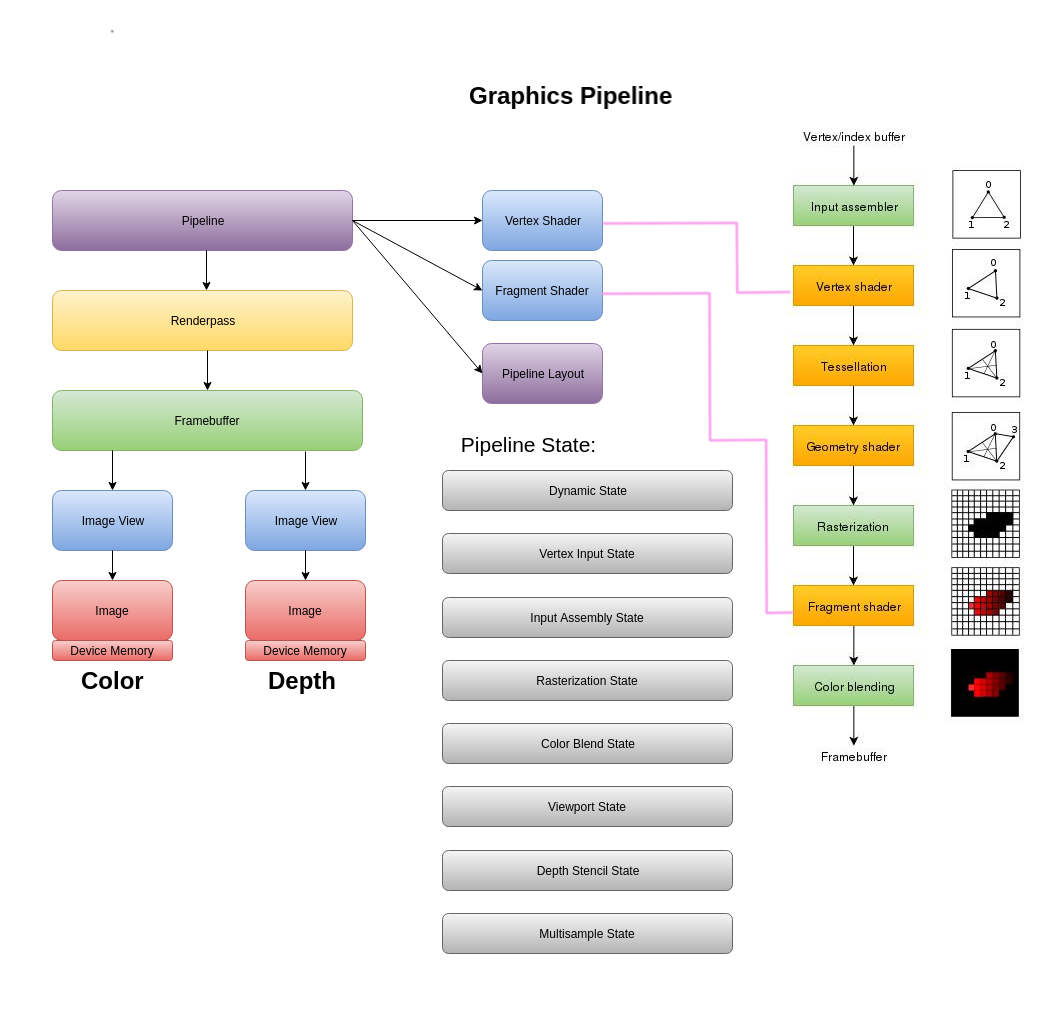
\includegraphics[scale = 0.4]{images/pipeline.png}
        \caption{Vulkan Pipeline}
    \end{figure}

    管线状态中:

    \begin{itemize}[itemindent=1em]
        \item dynamic state 是用来确定 uniform 变量数据的阶段;
        \item vertex input state 则是从内存输入顶点到着色器的阶段,
                这个阶段会看 layout 关键字指定的着色器数据,并且将顶点数据给着色器;
        \item input assembly state 则是告诉 GPU 需要将输入的点都按照什么样的形状连在一起(三角形,直线,点);
        \item rasterization state 则决定如何光栅化;
        \item color blend state 决定如何进行颜色混合(是不是用透明色,颜色空间如何);
        \item viewport state 则指定了屏幕的视口和大小;
        \item depth stencil state 会对图像进行深度和模板测试;
        \item Multiplesample 是多重采样,指定如何使用采样和抗锯齿。
    \end{itemize}


\clearpage
\subsection{着色器模块}
    与传统图形 API 不同,Vulkan 中的着色器代码必须以二进制字节码的格式使用,
    而不是像 GLSL 和 HLSL 这样具有比较好的可读性的语法。
    此字节格式称为 SPIR-V,它可以与 Vulkan 和 OpenCL 一同使用。
    这是一种可以编写图形和计算着色器的格式。
    值得注意的是,Vulkan spec 规定 SPIR-V 的代码长度必须是 4 的整数倍。

    GPU 厂商的编译器将字节码转换为原生代码的工作复杂度远远低于直接编译较高级的类 C 代码。
    过去的经验告诉我们使用类 C 代码,比如 GLSL 作为着色器代码,会因为不同 GPU 厂商对代码的不同解释而造成大量问题,
    并且类 C 代码的编译器实现要比字节码编译器复杂的多,GPU 厂商实现的编译器也极有可能存在错误,
    不同 GPU 厂商的实现也差异巨大。而使用字节码格式,上述的这些问题可以在极大程度上减少。

    但是,并不意味着我们要手写字节码。
    Khronos 发布了与厂商无关的编译器,它将 GLSL 编译成 SPIR-V。
    该编译器用于验证着色器代码是否符合标准,并生成与 Vulkan 功能运行的 SPRIR-V 二进制文件。
    除此之外还可以将此编译器作为库在运行时编译生成 SPRI-V。


\clearpage
\subsection{命令池}
    命令必须存放在命令缓冲里,命令缓冲必须由命令池创建和管理。
    每个命令池都与一个特定的队列族相关联。
    命令池用于分配和管理命令缓冲,以便在队列中执行命令。
    不同的队列族可能需要不同的命令池。


\clearpage
\subsection{命令缓冲}
    Vulkan 中的指令,例如绘制命令和内存传输命令并不是直接通过函数调用执行的。
    需要将所有要执行的操作记录在一个命令缓冲对象中,
    然后提交给可以执行这些操作的队列才能执行。
    因此,可以在程序初始化时就准备好所有要指定的指令序列,
    在渲染时直接提交执行。

    命令缓冲用于存储一系列的命令,包括渲染命令、资源操作命令等。
    命令缓冲由命令池分配,然后可以提交到队列中执行。
    每个命令缓冲都与一个特定的命令池和队列族相关联。

    \textbf{总结}:队列族定义了不同类型的队列,命令池用于管理命令缓冲,命令缓冲存储一系列的命令,
    而队列负责按顺序执行这些命令。通过这种组织和管理,Vulkan可以高效地执行渲染和计算操作,并充分利用多线程和并行处理的优势。


\clearpage
\subsection{顶点缓冲}
    顶点数据既可以直接写进 glsl 里,也可以通过 CPU 端传输到 glsl 里。
    后者需要使用顶点缓冲区来存放顶点数据。

    相关操作有:获取所需缓冲区内存大小、分配缓冲区、绑定顶点数据到缓冲区。


\clearpage
\subsection{帧缓冲}
    渲染得到的数据会写入附件中(颜色附件、深度附件等),然后存入帧缓冲中。




\clearpage
\section{进入事件主循环}
    渲染循环。




\clearpage
\section{清理资源并退出}
    销毁创建的资源,避免内存泄漏。


% \clearpage
% \section{直接输出图片到文件}
%     我们也可以完全不使用交换链,直接将帧缓冲中的数据输出到文件,然后使用 FFmpeg 命令查看。

%     此时代码的结构较为简单:

%     \begin{enumerate}[itemindent=1em]
%         \item 创建实例、物理设备(只需图形队列即可)、逻辑设备;
%         \item 创建颜色附件、SubPass(依赖)、RenderPass
%         \item 创建渲染管线(顶点输入描述、读取 shader);
%         \item 创建 VkImage,绑定 VkImage 到 VkDeviceMemory;
%         \item 创建 VkImageView、帧缓冲;
%         \item 创建顶点数据、顶点缓冲区、映射内存;
%         \item 创建命令池、命令缓冲区、记录命令(渲染等操作)
%         \item 渲染循环(记录命令,提交命令)。
%     \end{enumerate}

%     此时不涉及多个选子通道,因此不需要同步渲染命令。
\end{document}

    

% libvulkan.so 会根据 icd json 文件来选择调用哪一个厂商实现的驱动。
% 例如,libvulkan\_benbu.so

% 因此需要设置 export VK\_ICD\_FILENAMES=...../...icd.json
% 该 json 文件里就写明了厂商的 so 在哪里。

% 查看图像:ffplay -f rawvideo -pixel_format rgba -video_size 800*600 -i filename.rgba